%**************************************************************
\chapter{KALCAS: Un frameworK para evaluaci\'on de ALineamiento de arquiteCturAS de informaci\'on y procesos de negocio} \label{cha:solution}
%**************************************************************

%===============================================================
\section{Conceptualizaci\'on} \label{sec:conceptualization}
%===============================================================
Definimos formalmente los conceptos de alineaci\'on y redundancia en t\'erminos de los elementos de BA e IA con el objetivo de automatizar la tareas de comparar los elementos de cada dimensi\'on e inferir trazabilidad, las cuales fueron abordadas en el Cap\'itulo \ref{cha:intro}. Para el prop \'osito de este trabajo, asumimos la trazabilidad como un s\'intoma de alineaci\'on y la redundancia como una se\~nal de potencial desalineamiento.

El problema de identificaci\'on de trazabilidad BA-IA, podemos formalizarlo como una funci\'on entre los conjuntos de componentes que conforman estas arquitecturas.

\begin{theorem}
\label{def:traceability}
Sea ($C_{i}$) un componente de negocio, definimos que presenta trazabilidad con un componente de Informaci\'on ($C_{j}$) si tiene una correspondencia superior a un umbral de similitud ($TH$):
\begin{center}
\begin{math}
traceability(C_{i},C_{j}) \Longrightarrow C_{i} \in BA \wedge C_{j} \in IA \wedge sim(C_{i},C_{j}) \geq\ TH
\end{math}
\end{center}
\end{theorem}

Por otro lado, la definici\'on de redundancia dentro de los elementos de cada dominio, la entendemos como la relaci\'on de semejanza entre componentes del mismo dominio.

\begin{theorem}
\label{def:redundancy}
Sean ($C_{i}$ y $C_{j}$) componentes dentro del mismo dominio de EA cuyo \'indice de similitud superior a un umbral dado ($TH$): 
\begin{center}
\begin{math}
redundancy(C_{i},C_{j}) \Longrightarrow (C_{i}, C_{j} \in BA \vee C_{i}, C_{j} \in IA ) \wedge sim(C_{i},C_{j}) \geq\ TH
\end{math}
\end{center}
\end{theorem}

Estas definiciones nos permiten calcular que: El total de comparaciones de alineaci\'on est\'a dado por el producto cartesiano ($M \times N$), donde $M$ es la cantidad de elementos de $BA$ y $N$ la cantidad de elementos de $IA$. La cantidad de verificaciones de redundancia est\'a dada por el coeficiente binomial $\frac{{n!}}{2!(n-2)!}$, donde $n$ es la cantidad de elementos a contrastar en cada dominio ($M$ o $N$). De lo anterior se concluye que el orden de complejidad algor\'itmico de la funci\'on $traceability$ es de la forma $O(m \times n)\simeq O(n^2)$. El orden de complejidad de la funci\'on $redundancy$ es de la forma $O(\frac{n^2}{2}) \simeq O(n^2)$. Por tanto las dos funciones tienen un orden de complejidad cuadr\'atico lo que nos permite decir que son \textit{abordables} desde el punto de vista computacional.

Con las definiciones de \textit{traceability} y \textit{redundancy} podemos ahora proponer nuestra definici\'on de alineaci\'on entre BA-IA:

\begin{theorem}

\label{def:alignment}
Sea ($C_{i}$) un componente de negocio o Informaci\'on, definimos que est\'a potencialmente alineado si presenta trazabilidad con  elementos de otro dominio y no incurre en redundancia con elementos del dominio:
\begin{center}
\begin{math}
alignment(C_{i}) \Longrightarrow C_{i} \in traceability(C_{i},C_{j}) \wedge C_{i} \notin redundancy(C_{i},C_{j})
\end{math}
\end{center}
\end{theorem}


%===============================================================
\section{Extensiones al metamodelo Tartarus}
%===============================================================

Como parte de nuestro trabajo, extendimos el metamodelo de procesos de negocio e informaci\'on, con el prop\'osito de expresar las correlaciones que se pueden dar entre los diferentes elementos. Los \textit{Match Elements} se pueden observar en la parte inferior de la Figura \ref{fig:BA-IA-MM} y las relaciones de estas metaclases con las funciones de trazabilidad y redundancia se detallan en la Figura \ref{fig:Aling_Redund_mm}.

%........................................................


\begin{figure} [!t]
\begin{center}
	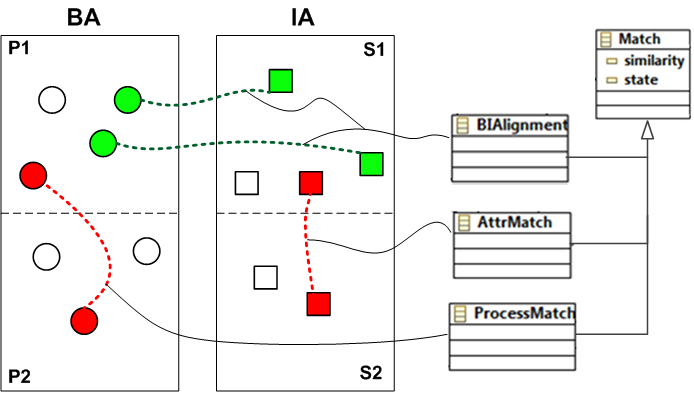
\includegraphics[scale=0.45,natwidth=694pt, natheight=398pt]{Aling_Redund_mm.png}
	\caption{Expresi\'on de Trazabilidad y Redundancia sobre las Extensiones del Metamodelo Tartarus}
	\label{fig:Aling_Redund_mm}
\end{center}
\end{figure}
%........................................................

La superclase \textit{Match} representa las correspondencias tanto de componentes dentro el mismo dominio (posibles redundancias) como de dominios diferentes (posibles alineaciones) asignando un \'indice de similitud y el estado de revisi\'on (\textit{PENDING} o \textit{VERIFIED}). Esta clase se especializa en cada tipo de mapeo: \textit{AttrMatch} asocia pares de \textit{Attribute} de diferentes esquemas, por ejemplo, una coincidencia entre la entidad \textit{S1.REGISTRATION} y \textit{S2.REGISTERED}. De una manera an\'aloga \textit{ProcessMatch} representa coincidencias potenciales entre pares de \textit{ProcessElement} por ejemplo, entre las actividades \textit{P1.Register} y \textit{P2.Migrate Registration}. Finalmente, la subclase \textit{BIAlignment} permite vincular los dominios de Informaci\'on y Negocio (alineamiento BA-IA) mediante la asociaci\'on directa entre objetos \textit{Abstract} y \textit{DataObject}.


%===============================================================
\section{Estrategia}
%===============================================================

El n\'ucleo de nuestra aproximaci\'on es el modelo Tartarus de la organizaci\'on, donde est\'an expresados formalmente los componentes de la EA, es decir los conjunto de IA y BA. El objetivo central es definir los conjuntos de BA e IA y aplicar las funciones de alineaci\'on y redundancia utilizando un motor de alineamiento de ontolog\'ias para inferir \'indices de similitud entre los elementos de ambos conjuntos.

Nuestra estrategia para inferir trazabilidad y detectar desalineaciones consta de cinco fases, cada una de las cuales es soportada por herramientas construidas dentro de este trabajo. El usuario participa verificando los mapeos candidatos inferidos autom\'aticamente por el motor de matching (de all\'i que nuestra aproximaci\'on es semi-autom\'atica) y realizando consultas de alineamiento sobre el modelo utilizando nuestro DSL gr\'afico KQL que se detallar\'a en el Cap\'itulo \ref{cha:KQL}. Una vista general de nuestra propuesta de soluci\'on se muestra en la Figura \ref{fig:Solution}.

%........................................................
\begin{figure} [!t]
\begin{center}
	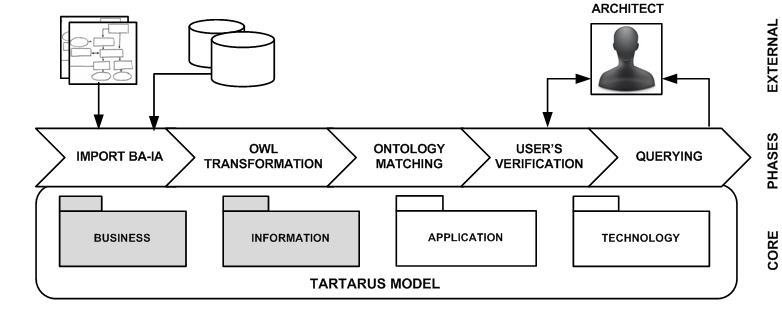
\includegraphics[scale=0.7,natwidth=782pt, natheight=309pt]{Solution_Overview2.png}
	\caption{Vista General de la Soluci\'on}
	\label{fig:Solution}
\end{center}
\end{figure}
%........................................................


%===============================================================
\subsection{Importar arquitecturas de negocio e informaci\'on}
%===============================================================

Inicialmente se requiere identificar los elementos de cada dimension de la EA, para tal fin, se importan mediante una herramienta que puebla el modelo, desde un archivo XML Process Definition Language (XPDL) para la BA o v\'ia JDBC (base de datos relacional) para la IA. Los archivos XPDL son importados mediante un \textit{serializer} desarrollado en \cite{Rodriguez:2011} el cual utiliza la librer\'ia \textit{XStream} que serializa objetos a XML y viceversa. A la versi\'on preliminar se agregaron conversores de \textit{Data Objects}, elementos necesarios en la inferencia de los alineamientos en nuestra propuesta. Los esquemas se acceden a trav\'es de una conexi\'on JDBC. Se obtiene la metadata utilizando las facilidades ofrecidas dentro del paquete \textit{java.sql}. 

En esta fase, tanto los elementos de cada conjunto, como sus estructuras y la metadata asociada son incorporados en las descripciones formales, a fin de obtener modelos enriquecidos que favorezcan las inferencias. El modelo Tartarus es creado y poblado program\'aticamente utilizando a trav\'es de las librer\'ias java que ofrece Eclipse Modeling Framework (EMF). Para el caso del ICFES, se obtiene el modelo \textit{ICFES.tartarus} expresado en conceptos Tartarus y una vista de los principales elementos del modelo se muestran en la Figura \ref{fig:icfesmodel}. 

%........................................................
\begin{figure} [!t]
\begin{center}
	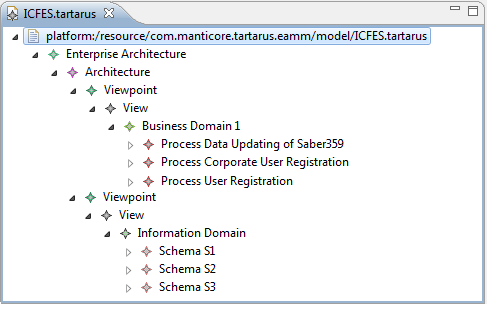
\includegraphics[scale=0.75,natwidth=487pt, natheight=307pt]{ICFEStartarus.png}
	\caption{EA del ICFES Importada al modelo Tartarus}
	\label{fig:icfesmodel}
\end{center}
\end{figure}
%........................................................

%===============================================================
\subsection{Transformaciones OWL}
%===============================================================
Posteriormente, se ejecuta una transformaci\'on Xpand \cite{Xpand:2006}, para para llevar todas las definiciones consignadas en el modelo Tartarus a ontolog\'ias OWL. Se genera un archivo OWL por cada esquema y proceso contenido en el modelo Tartarus. Para el caso del modelo \textit{ICFES.tartarus}, se generan cuatro ontolog\'ias: \textit{S2.owl}, \textit{S1.owl}, \textit{User Registration.owl} y \textit{Corporate User Registration.owl}.

La Tabla \ref{tab:tartarusowl} resume las correspondencias entre las clases Tartarus y los elementos OWL en cada uno de los dominios. En el modelo de procesos de negocio, todos los elementos de tipo \textit{ProcessElement} (Activity, SubProcess, Gateway, DataObject y Event) son transformados a clases OWL (\textit{owl:Class}). Por otra parte, los elementos de clase \textit{Connection} se convierten en objetos \textit{owl:ObjectProperty} que vinculan los \textit{ProcessElement}. 


\begin{table}
\begin{center}
\scalebox{1}{
\begin{tabular}{c c c} \hline
Dominio & Concepto Tartarus & Elemento OWL\\
\hline
IA & Schema & OWL File \\
IA & Abstract & \textit{owl:Class} \\
IA & SimpleAttribute & \textit{owl:DataProperty} \\
IA & BinaryAbstractAggregation & \textit{owl:ObjectProperty} \\
IA & Attribute.remarks & \textit{rdfs:comment} \\
IA & Remarks & \textit{rdfs:comment} \\
\hline
BA & Process & OWL File \\
BA & Actitivity & \textit{owl:Class} \\
BA & DataObject & \textit{owl:Class} \\
BA & Gateway & \textit{owl:Class} \\
BA & Event & \textit{owl:Class} \\
BA & Connection & \textit{owl:ObjectProperty} \\
BA & ProcessElement & \textit{owl:Class} \\
BA & Remarks & \textit{rdfs:comment} \\
\end{tabular}
}
\end{center}
\caption{Transformaciones de Conceptos Tartarus a Elementos OWL}
\label{tab:tartarusowl}
\end{table}

En el dominio de informaci\'on, cada objeto \textit{Abstract} es traducido a un \textit{owl:Class}. Los elementos \textit{SimpleAttribute} son mapeados como \textit{owl:DatatypeProperty} de la clase OWL contenedora. El tipo de dato de dichos atributos es redefinido como dato \textit{XMLSchema} primitivo. Sumado a esto, si el atributo est\'a marcado como \textit{isId}, un elemento \textit{owl:FunctionalProperty} es incluido. Los atributos de tipo \textit{Abstract} son transformados a elementos \textit{owl:ObjectProperty}, donde el dominio es la clase contenedora y el rango corresponde al atributo \textit{Abstract}. Las instancias de \textit{BinaryAbstractAggregation} tambi\'en se convierten en \textit{owl:ObjectProperty}, donde los \textit{Abstract} origen y destino se homologan a dominio y rango respectivamente. Los comentarios o metadata disponible tanto para procesos como para entidades, son incluidos en las ontolog\'ias de salida en la forma de \textit{rdfs:comment}. La Figura \ref{fig:Transform} ejemplifica como son transformados algunos de los elementos de \textit{ICFES.taratus} a ontolog\'ias owl.

%........................................................
\begin{figure*}[!t]
\begin{center}
	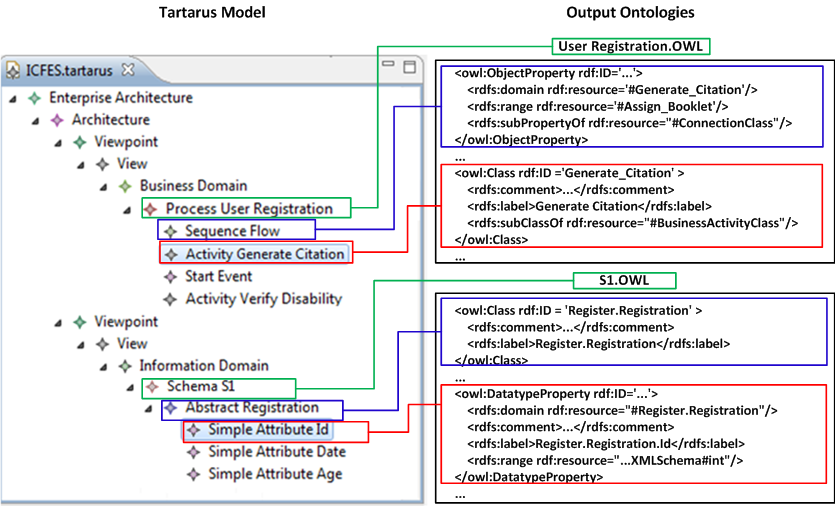
\includegraphics[scale=0.6,natwidth=835, natheight=506pt]{OWL_trans.png}
	\caption{Ejemplo de Transformaci\'on Tartarus-OWL}
	\label{fig:Transform}
\end{center}	
\end{figure*}
%........................................................
%===============================================================
\subsection{Matching de Ontolog\'ias} \label{sec:alignstep}
%===============================================================
En esta fase se infiere la trazabilidad y redundancia en los dominios BA-IA. Se procesan mediante un motor de matching las ontolog\'ias generadas en el paso anterior. Definimos dos tipos de tareas de matching de ontolog\'ias en el \'ambito de Kalcas: Entre ontolog\'ias de dominios diferentes y entre ontolog\'ias del mismo dominio. Estas dos tipolog\'ias est\'an en l\'inea con las funciones $traceability(C_{i},C_{j})$ y $redundancy(C_{i},C_{j})$ definidas en la Secci\'on \ref{sec:conceptualization}. La Figura \ref{fig:alignmenttask} muestra la ejecuci\'on de los dos tipos de tareas de alineamiento.

%........................................................
\begin{figure} [!t]
\begin{center}
	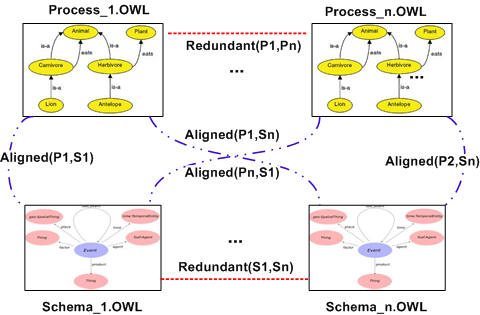
\includegraphics[scale=0.55,natwidth=480, natheight=315]{Schema_Alignment.png}
	\caption{Tipos de Tareas de Matching de Ontolog\'ias en Kalcas}
	\label{fig:alignmenttask}
\end{center}	
\end{figure}
%........................................................


La arquitectura de Kalcas utiliza el motor de alineamiento como un componente de software, por tanto es independiente a la implementaci\'on del motor de matching de ontolog\'ias. El motor de alineaci\'on utilizado en la versi\'on actual de Kalcas es \textit{Alignment API 4.3} disponible en \cite{AlignmentAPI:2012}. Esta API es una implementaci\'on para expresar, ejecutar y compartir alineamientos de ontolog\'ias \cite{David:2011}. Para cada pareja de ontolog\'ias, invocamos program\'aticamente \textit{Alignment API}, seleccionando un conjunto de comparadores que ya vienen implementadas dentro del API. Cada algoritmo debe ser configurado con par\'ametros como umbral de similitud. Estas t\'ecnicas, utilizan nombres, comentarios, etiquetas, tipos de dato y estructuras para determinar un grado de similitud (entre 0 y 1). Las correspondencias encontradas entre \textit{Abstract} y \textit{DataObject} son propagadas a las actividades asociadas a los \textit{DataObject} con el fin de trazar un puente entre actividades y entidades.

Todos los mapeos candidatos generados por el motor, son cargados de vuelta al modelo \textit{ICFES.tartarus} como elementos \textit{AttrMatch, ProcessMatch o BIAlignment} utilizando EMF en un estado pendiente (\textit{state=PENDING}) y con el \'indice de similitud calculado por el motor. Por ejemplo, la correspondencia inferida entre las entidades \textit{S1.Registration} y \textit{S2.Registered} es consignada en el modelo como el objeto \textit{AttrMatch : S1.Registration\_ S2.Registered} con atributos: \textit{left:S1.Registration, right:S2.Registered, sim:0.9, state:PENDING}. 

%........................................................
\begin{figure} [!t]
\begin{center}
	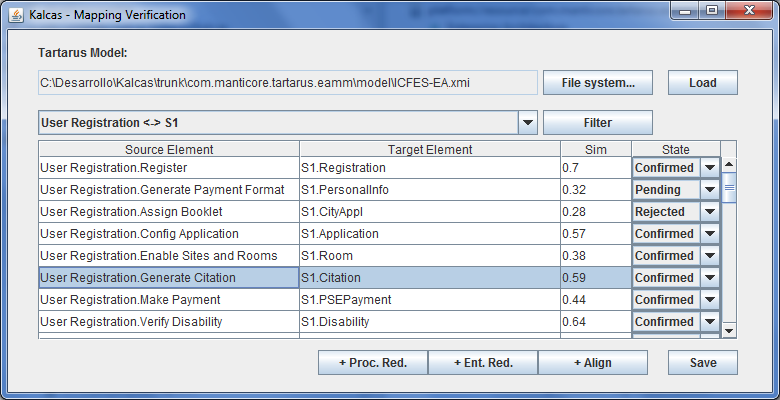
\includegraphics[scale=0.65,natwidth=783, natheight=399]{guiuser.png}
	\caption{GUI para Verificaci\'on de Mapeos Candidatos}
	\label{fig:Confirmation}
\end{center}	
\end{figure}
%........................................................

%===============================================================
\subsection{Verificaci\'on de Usuario}
%===============================================================

Una vez calculadas las alineaciones y redundancias candidatas, estas deben ser verificadas por el arquitecto.  Para tal fin, una interfaz gr\'afica de usuario (GUI) fue desarrollada con la librer\'ia Swing de Java y EMF para acceder y actualizar el modelo. Esta GUI permite seleccionar el modelo Tartarus, y una vez cargado se presenta una tabla con las correspondencias inferidas y su \'indice de similitud. El usuario puede confirmar o rechazar el mapeo como se ve en la Figura \ref{fig:Confirmation}. El prop\'osito de esta interfaz es ofrecer facilidades como filtros y ordenamientos para la gesti\'on de los mapeos candidatos. 

Tras la verificaci\'on del experto, los mapeos quedan en estado \textit{CONFIRMED} o \textit{REJECTED} dentro del modelo Tartarus. S\'olo los mapeos con confirmados son tenidos en cuenta en las consultas posteriores sobre el modelo.

